In this section, we take a close look at the proposed structure and capabilities of the framework.
We will then discuss the implementation and its difficulties.

\section{Proposed Functionality}

The framework shall have two primary capabilities: first, it should enable fast and easy access to the 3d homography calculated from the marker.
Second, given a model to display, it should be capable of returning a rendering of the object within the scene on top of the live preview.

Generally, the framework shall work as in the following.
Once the framework is running, OpenCV reads the camera frame directly from the camera.
This frame is copied to the worker threads that will detect markers.
The original unaltered frame is passed back up to be shown as the background of the later rendering.

These worker threads are where the computational expensive part of actually detecting the marker happens.
Using the Android Java port of the OpenCV library, we detect markers and calculate their homography.
All detected markers are put into a list with the important deducted information, such as the corresponding identification number of the detected marker.

This list is passed back to the main controlling element of the framework.
Here it can be passed directly to listening classes if that option was chosen.
If not, the list is filtered for only those markers that the user wants to track (meaning any that were registered beforehand).
Then the model information is attached to all detected trackable assets and passed down to the rendering part of the framework.
Here, this filtered and supplemented list is used to render all objects onto the correct positions with the correct perspective modifications on top of the camera feed.

Apart from the above mentioned basic functionality capabilities, the framework should also handle the easy gathering of performance and error information, mainly be extending the relevant functions of Android.
This can include gathering the logs to a listener, bypassing the Android logging mechanism, and any further functionality that could be useful.

\begin{figure}
	\centering
	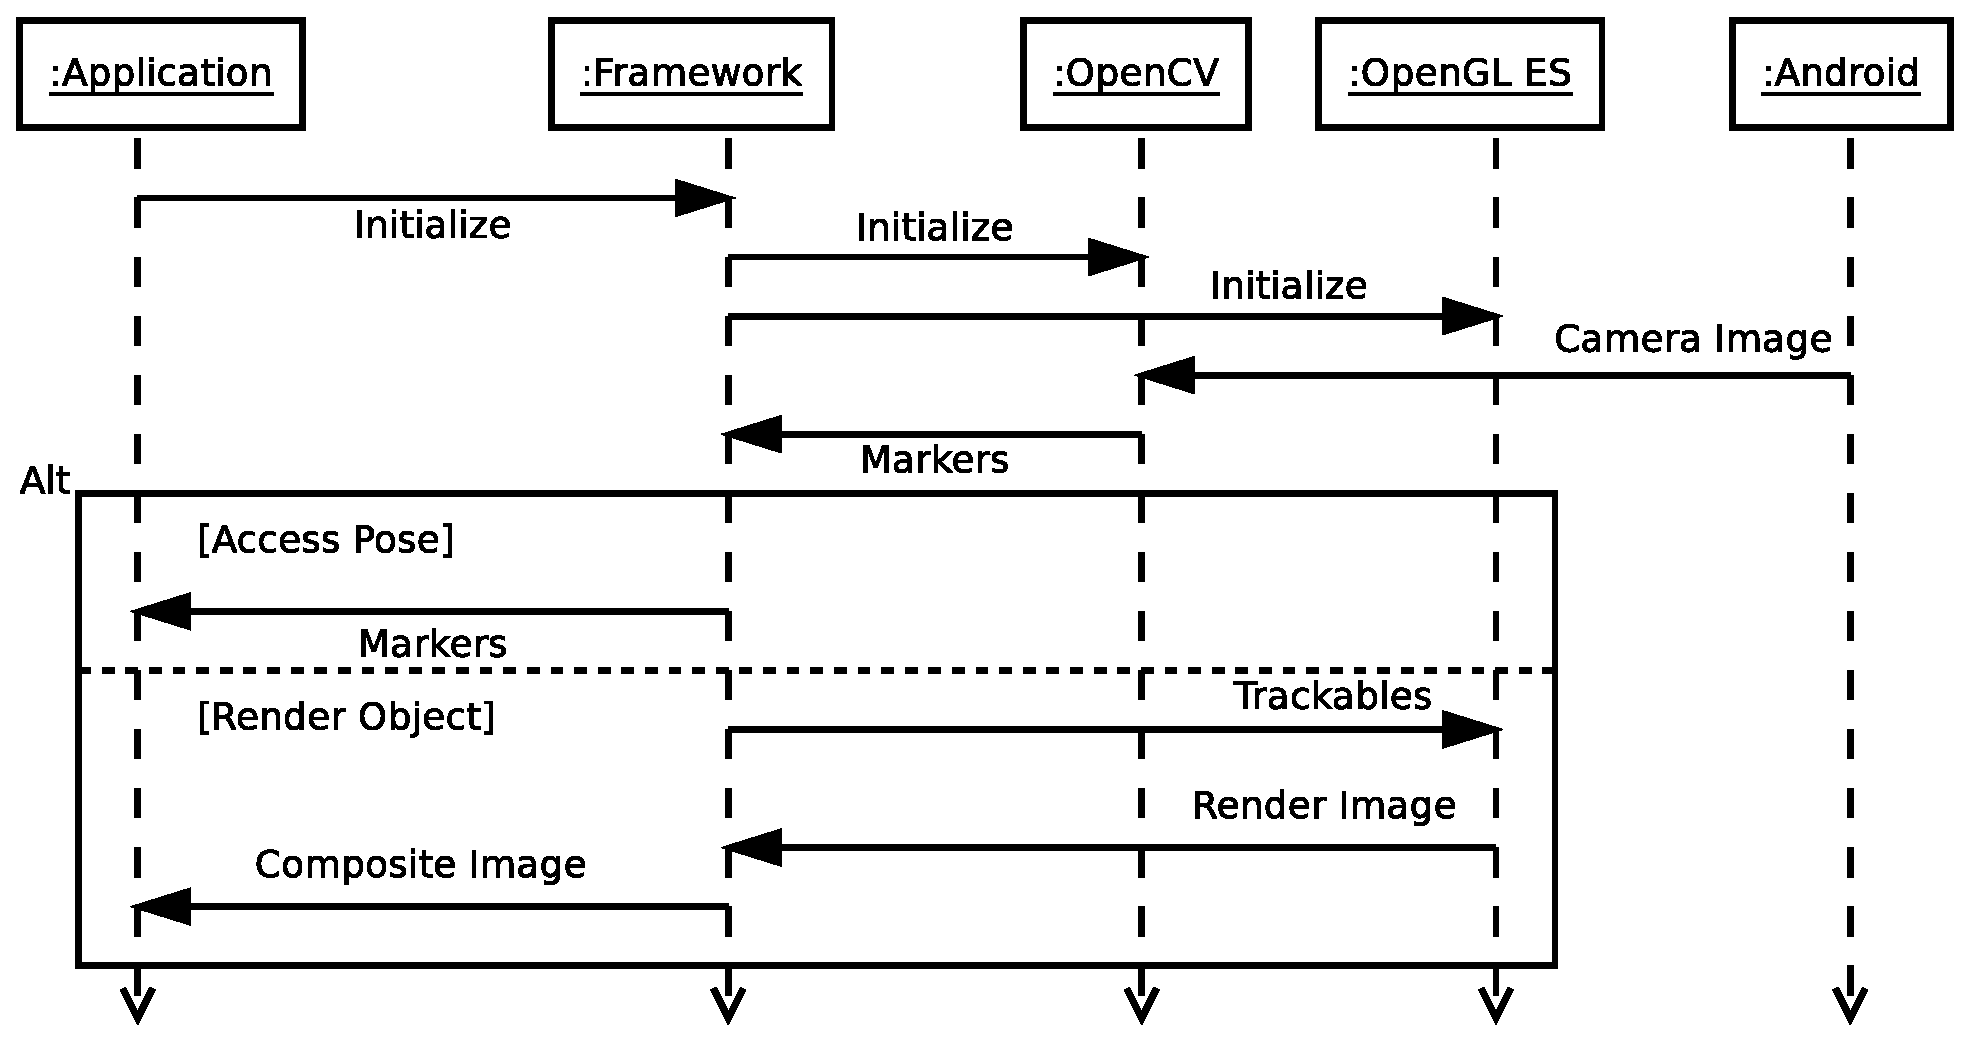
\includegraphics[width=12cm]{img/sequence_access.eps}
	\caption[TODO Access Sequence.]{The proposed sequence of the workflow with the framework, using OpenCV.}
	\label{fig:sequence_access}
\end{figure}

Figure \ref{fig:sequence_access} shows the proposed outside view of the framework, and where data can be input or read.
As proposed, the framework should offer a wide variety of uses, without being overly complex from an outside perspective.
Another important aspect we want to make possible is the possibility of changing all the more important parameters during runtime, such as switching the model or adding a new marker.
This should allow a less restrictive usage of the framework and any derived apps as a result.

\section{Dependencies}

Primary dependency is of course an Android environment, given that it is the target platform for the framework.
The framework is written in Java with the Android dependencies used.
Aside from the basic requirements, the framework will depend mainly on two external software solutions.

The first is OpenCV\cite{opencv}, an open source collection of computer vision and machine learning software.
The framework makes use of the Java-based port.
To use the framework on Android, the OpenCV Manager\cite{opencvmanager} needs to be installed alongside the app using the framework, as the marker detection relies on it.
The OpenCV manager offers the best version for each Android device according to its specifications and capabilities.

Apart from OpenCV, OpenGL ES is used for the rendering of the 3D objects to the display.
For this dependency, nothing has to be considered from an app that would use the framework, as the mobile version of OpenGL is already built into Android.
According to the capabilities of the developer device used, we chose to use OpenGL ES 2.0.
We chose not to go with version three because at this time, a minority of devices support it and we lack access to a device capable of it.\footnote{TAMINO TODO: Add OpenGL 2.0 stuff that might be important. Why not use 1.1 etc...}

\section{Limitations of Scope}

In the following we will look at the features required of the framework to be considered complete.
Some nice-to-have features will also be listed, meaning features that will not be implemented but could possibly be interesting for future further work.
For completeness, we will also take a short look at features that are possibly too difficult to do and or would require significant work.

To clarify the scope of the proposed framework, all features that will be delivered are described within the following table.
Note that while these are the main features, aspects of them might change for the implementation.

\begin{tabulary}{\textwidth}{L || L}
Debug Messaging & The framework should be easy to debug and allow simple access to status messages.\\
\hline
Manage Trackers & Allow to add and remove trackers during runtime.\\
\hline
Read Raw Data & Give the possibility of accessing the raw data returned from the OpenCV Wrapper so that custom solutions can be built without changing the source code.\\
\hline
Configuration & Allow easy visualization for various aspects of the framework.\\
\hline
Multi-threading & Allow computationally expensive tasks to run multi-threaded.\\
\end{tabulary}

The features in the following table are features that might be implemented, if their development proves to be beneficial to the framework and are easy enough to be added along the sidelines.

\begin{tabulary}{\textwidth}{L || L}
Animated Objects & Allow the object to have an animation and offer control access to it.\\
\hline
Simple Advanced Rendering & Possibly add some simple extra rendering features.\\
\end{tabulary}

The following are features that will not be implemented.
However, where possible, the framework will allow easy adaption to extend its functionality beyond what it will offer from the start.

\begin{tabulary}{\textwidth}{L || L}
Marker-less Tracking & Marker-less tracking will most likely not be within the scope of the initial framework\footnote{TODO: See also section ~ }.\\
\hline
Occlusion & The capability to detect where scene occlusion is taking place is definitely beyond the scope of the framework, as this requires extensively more work.\\
\hline
Fancy Rendering & No support for stereoscopic rendering. Depending on the difficulty of implementation, support for different direct rendering engines within the framework might be included which would allow an easy way of adding this functionality.\\
\end{tabulary}

\section{Class Diagram}

\begin{figure}
	\centering
	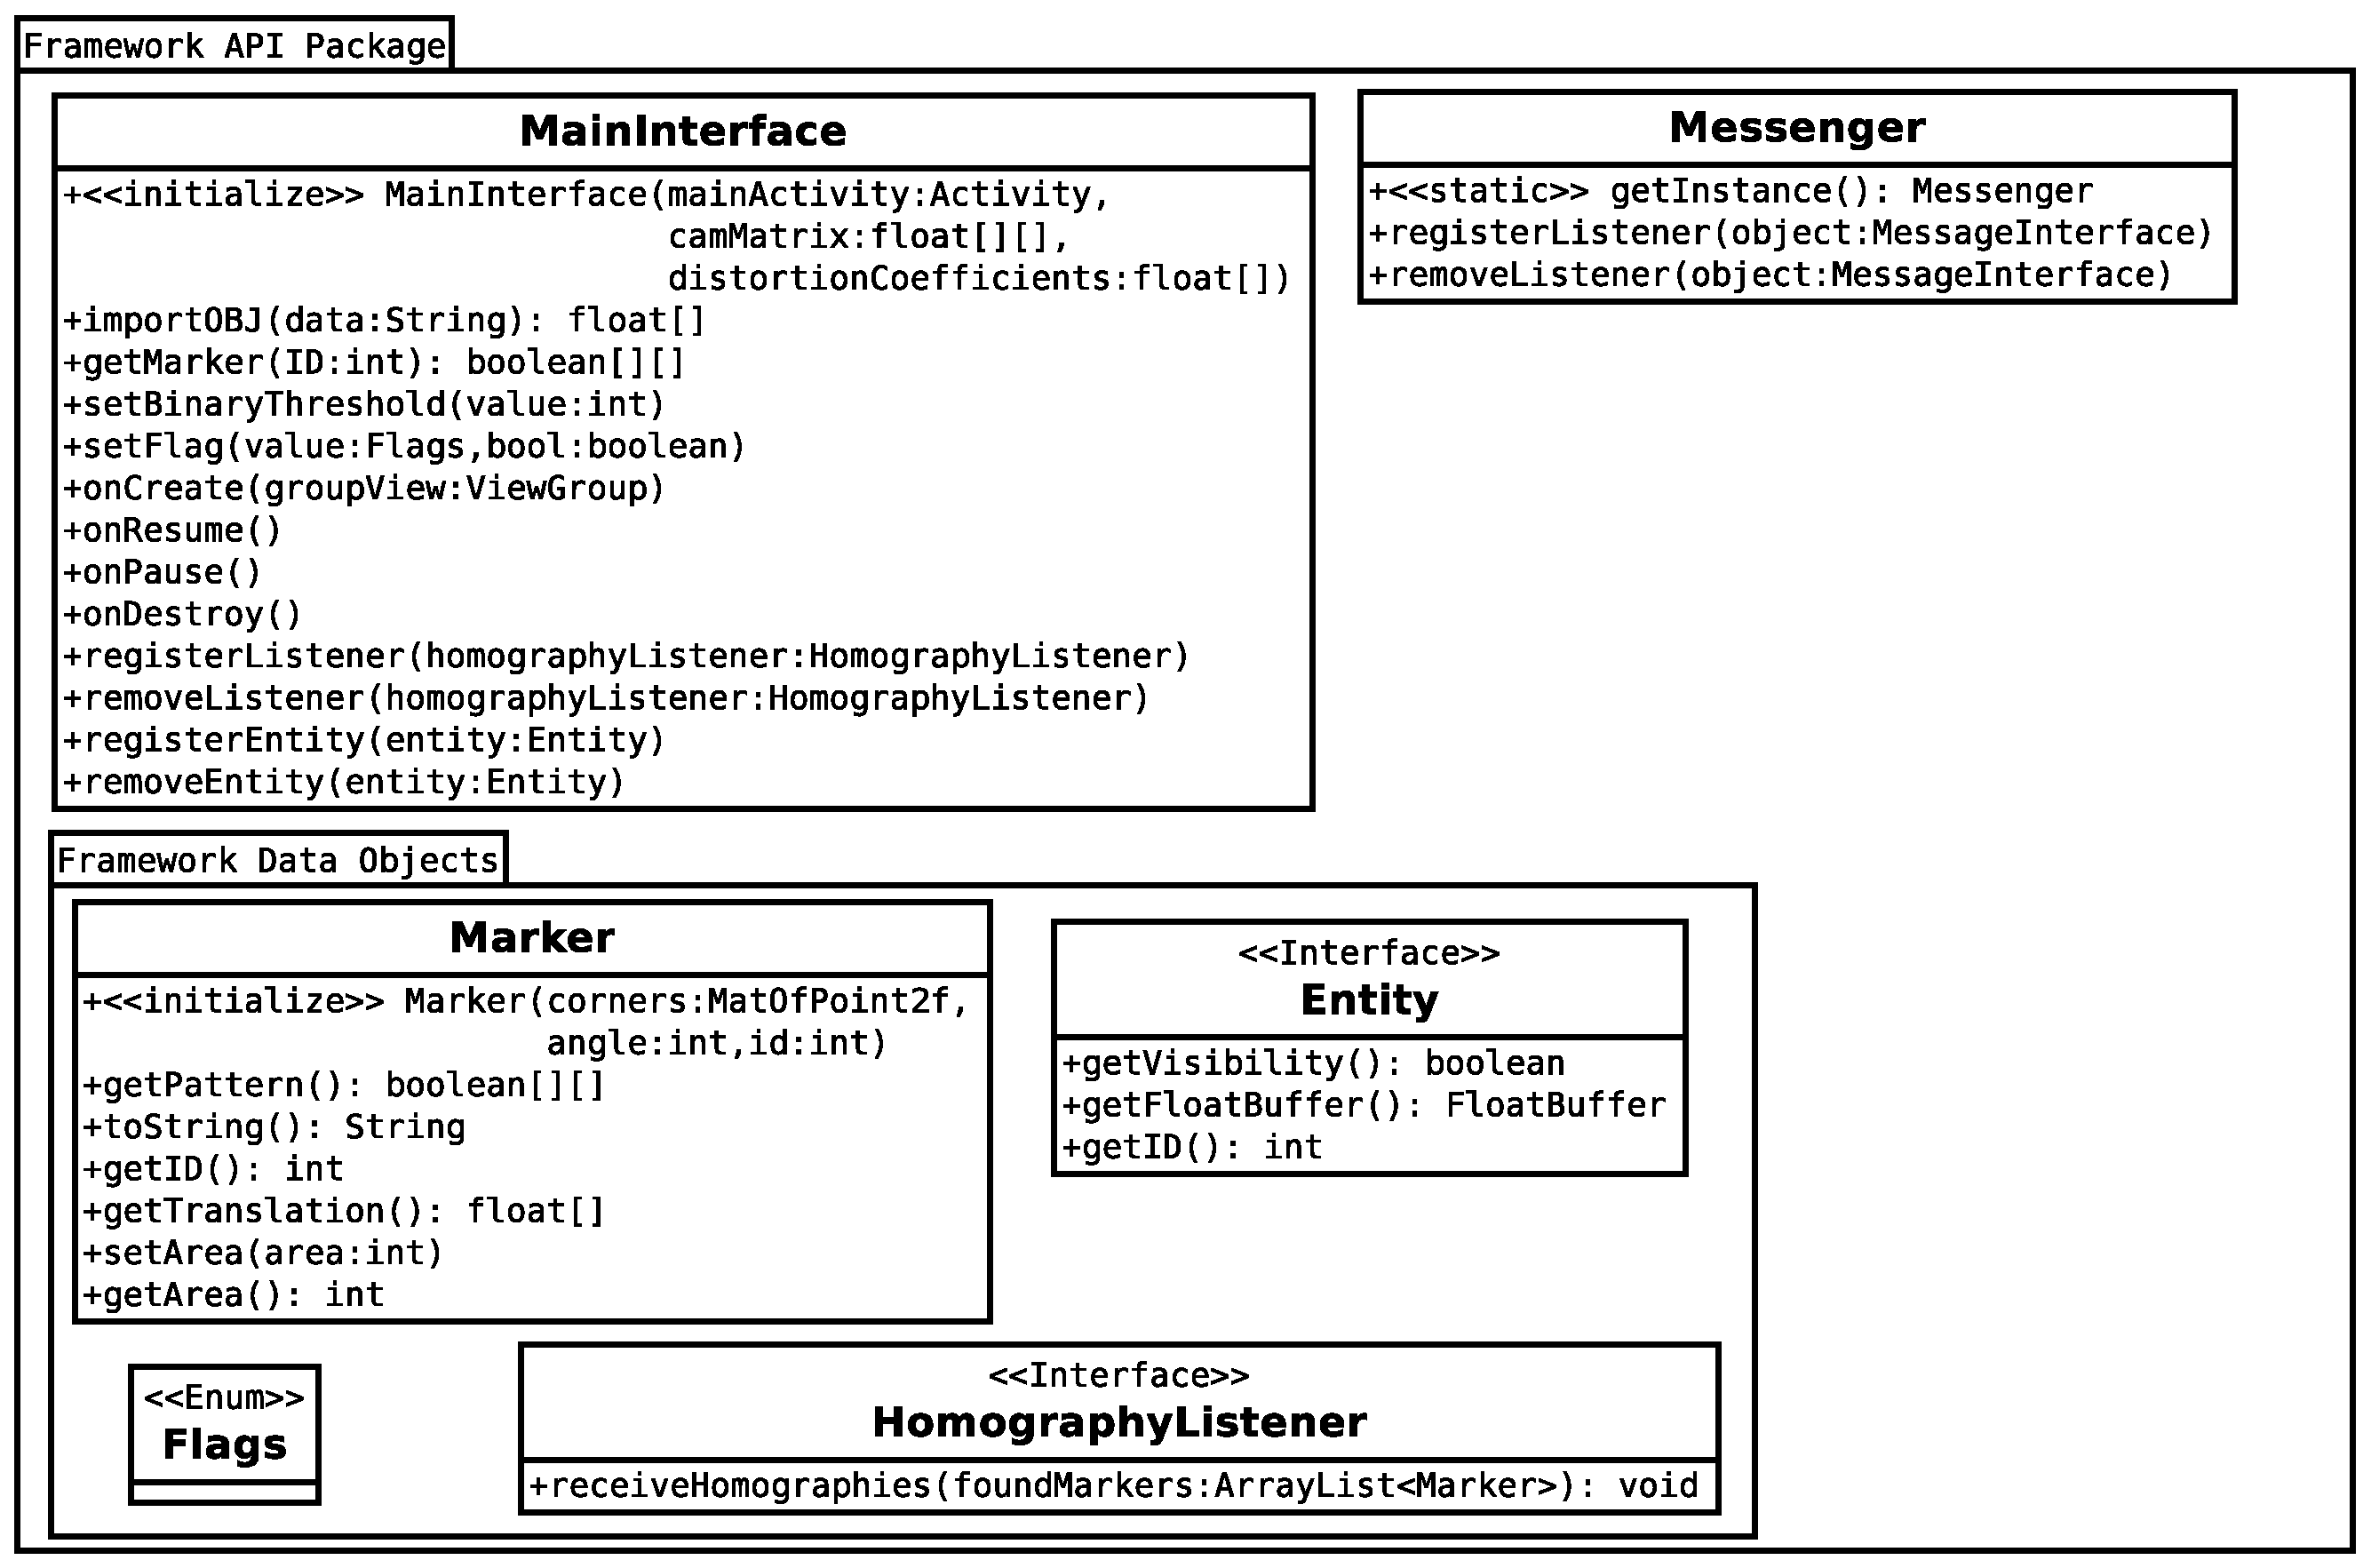
\includegraphics[width=10cm]{img/class_diagram.eps}
	\caption[TODO General Class Diagram]{This is the preliminary class diagram of the proposed functionality of the framework. Note the low number of public methods: this should make usage of the framework very easy. Also note that the Messenger class has no dependencies towards other classes to enable it to run as a distraction-free subthread from the rest of the framework.}
	\label{fig:class_diagram}
\end{figure}

Now let us take a look at the proposed class structure of the framework, as seen in Figure \ref{fig:class_diagram}.
Main access is controlled over the framework controller, which almost exclusively contains all the public methods callable from outside of the framework.
Apart from the framework controller, some model classes are also accessible as public classes to ease data transfer (notably for example the marker class so that little effort has to go into data conversion).

The messenger class allows easy and quick access to any debugging, logging, or error messages to outside classes via a listener principle.
This allows outside threads to be directly notified when a message is written and allows the end user to expand on any messages from the framework.

The Controller encapsulates all the primary functionality within the framework.
Apart from managing all the other classes on startup and closure, it also handles the information exchange between them and the caller, rendering all of these invisible to the outside program.
It also enables the management of the trackables and their assigned renderables\footnote{TAMINO TODO: Rework wording, might want to define in glossary too.}.
The Controller also handles any inter-system compatibility that the passage of information between the Renderer and Wrapper require.

The OpenGL ES Renderer class handles the generation of the images for the output in the form of a canvas.
It takes the 3d coordinate system from the OpenCV wrapper and renders the objects with the given specifications onto the  canvas over the camera feed.

Last is the OpenCV Wrapper. The Wrapper handles the control of the OpenCV library and does any managing work required for the framework.
This mainly includes the management of the worker threads that contain the marker detection algorithm.

The above proposed system should enable an easily extensible build for the framework while retaining a simplistic use case.
It should, in theory, be relatively easy to exchange either the worker threads or the render class to enable the framework to run beyond Android.
That would enable the framework to run on normal personal computers using the full-fledged version of OpenGL or possibly DirectX.

\section{Application Programming Interface}

The following represents the suggested interface for the framework.
With the listed methods, all functionality that the framework offers can be accessed.

{\footnotesize
\begin{tabulary}{\textwidth}{J || J}
<Initialization> & Constructs all the internal classes and prepares the major functionality. Also used to set the most important values such as camera distortion and camera perspective, as these are crucial for a correct processing. Furthermore also used to set the output layout where the results are drawn to.\\
\hline
onCreate & Must be called in the activities onCreate; handles all the necessary calls within the framework.\\
\hline
onResume & Must be called in the activities onResume.\\
\hline
onPause & Must be called in the activities onPause.\\
\hline
onDestroy & Must be called in the activities onDestroy.\\
\hline
registerListener & Add a homography listener. Listeners will be called if the correct flag has been set. Listeners will receive a list of detected markers containing all information.\\
\hline
removeListener & Removes a homography listener. \\
\hline
registerEntity & Adds an entity containing the ID, visibility status, and vertice buffer. This means that upon detection of the corresponding marker, the object will be rendered on top of it, according to the status of the visibility.\\
\hline
removeEntity & Removes an entity from the list.\\
\hline
setDebugFlag & Sets the given debug flag. For possible flags please see the Javadoc.\\
\hline
removeDebugFlag & Unsets the given debug flag.\\
\end{tabulary}
}

Important to note is that the onCreate, onPause, onResume, and onDestroy methods are inherent to the way programs work on Android, and thus must be called for the framework to function correctly.

Upon initialization of the framework, entities can be added to be tracked and rendered with the registerEntity method.
To do that, the user has to implement the entity interface, providing functionality for reading the identification that the object is to be bound to, whether it is to be rendered (the visibility option), and finally a FloatBuffer containing the vertice location and color information.
The use of the FloatBuffer might not seem intuitive at first glance, however that allows the framework to handle the rendering all on its own, greatly simplifying the usage of the framework.

\section{Usage}

The finished framework can track multiple markers in a single instance.
In fact, it tracks all markers it finds from the beginning, only filtering out the ones that the user is interested in before rendering.
This allows comparatively easy use of multiple, separately tracked entities.
However, this also has a significant drawback: as the framework is computationally expensive, multiple markers can quickly degrade its performance, even if the user only is interested in a single marker.
Therefore we suggest care considering the placement of unused markers to maximize performance.

For the tracking to work, the marker must be visible to the camera.
The marker can be shown on a separate screen, printed on paper, or drawn.
The framework will then detect the presence of the marker, continue with its identification and perspective information, and finally store it as a successfully detected marker for the render interface to render.
Utilizing the thus calculated perspective information, paired with the correct object, the renderer then proceeds to render objects onto their respective markers.

Concerning the placement and creation of the marker a few points should be considered.
First off, the framework offers a helper method for creating a binary representation of a marker given an identification number.
This removes any need for the user to manually create and encode a marker and the resulting marker is guaranteed to be correct.

Secondly, the marker should be black on white, with the black border contrasted by white space around it.
Correct detection of the presence of a marker can not be guaranteed otherwise.
Generally speaking, the framework is sensitive to the contrast range of the recorded camera feed, and thus it should be maximized.
Apart from monochrome markers, this also means that the environment should be brightly and constantly lit.

Thirdly, the marker should be created and printed digitally.
The correct detection of the border is the first and most important step in the detection of the marker and should thus be as good as can be managed.
While hand drawn markers can work, experimentation has shown that it is almost impossible to draw as accurate as required for the detection to be equal to printed markers.
This is only true for the border, however: the internal 4x4 grid containing the orientation and identification of the marker can be drawn in, so long as the drawing is done carefully.

\section{Implementation}

The following section describes in more detail the implementation of the framework.
First we implemented a test project to experiment with OpenCV on Android to collect data on possible solutions and problems.

At first, a feature-based approach was tried.
That meant that feature detection was used on the marker, resulting in a cloud of key feature points.
These can then theoretically be located in an image from which we have likewise extracted feature points.
However, this method proved to be too computationally expensive.
Initial tests only for detecting feature points in a live camera view already yielded framerates below 2 frames per second.
This was deemed insufficient for a realtime use of the finished product.

More research turned up a better solution based on the method used by the comparable Aruco\cite{aruco} framework.
The method was implemented as follows.

\subsection{Method for Tracking Markers}

The following is done each frame with OpenCV.
It results in a list of detected markers with their transformation matrices.

First, the input frame is transformed into a simple gray-scale image.
This gray-scale image is then processed into a monochrome image via an adaptive threshold method.
This results in clearly cut black and white areas that we can use in the next step.
We then extract all contours from the image.
These contours are used to fit polynomial approximations to all detected contours above a certain size.
We impose a size restriction to contours as we require a certain minimum size later when identifying the markers, and early exclusion of marker candidates speeds the process up significantly.
We can then filter the polynomial objects based on criteria for our markers, mainly for any contours that have 4 corners, are convex, and are a closed polynomial.

Now that we have a selection of detected perspective rectangles that might be markers, we sample all candidates for a black border.
Then we check for the orientation bits: if we find these, we can be comparatively sure that we have a valid marker and can continue to its identification.
If the detection of orientation fails (meaning that we do not find a pattern of three white and one black inner corner block), we consider the candidate to be invalid.
Now all that remains is the marker identification, which is done by sampling the remaining inside bits and error correcting them.
This process is further detailed in \ref{section_markers}\footnote{TODO: Maybe rework ordering? Is this answered in the linked section?}.

One of the major advantages of the polynomial representation of the markers is that it allows easy extraction of the homography required to calculate the 3d position of the markers.
Apart from that, it is also significantly faster – our first tests resulted in framerates of about 5 frames per second.

However, while 5 fps is better than 2 fps, it is still somewhat too slow for easy use.
Therefor, we suggest using multitasking to process multiple frames in parallel.
This allows the framework to run with around 7 fps.
This low increase may have a few reasons, of which the most likely is probably that OpenCV is currently not multi-threading capable.
As it does improve performance, we decided to keep it.

\section{How to Use}

Using the framework is very easy.
Simply create an instance of the MainInstance of the framework either in the constructor or in the onCreate method.
After creating the instance, call the onCreate method of the framework within the activity's onCreate.
To create the framework, it requires an Android GroupView where it will place the camera view and the view responsible for rendering the detected objects.
Now all that remains is to also call onPause, onResume, and onDestroy in the respective functions of the activity via the framework.
Now the parameters of the framework can be changed at any time, probably with event listeners.
